\subsection{Cache}
The cache will be utilized so that we do not have to make unnecessary requests to the connections when we are grabbing a user content on the respective service

\begin{figure}[h!]
	\centering
 	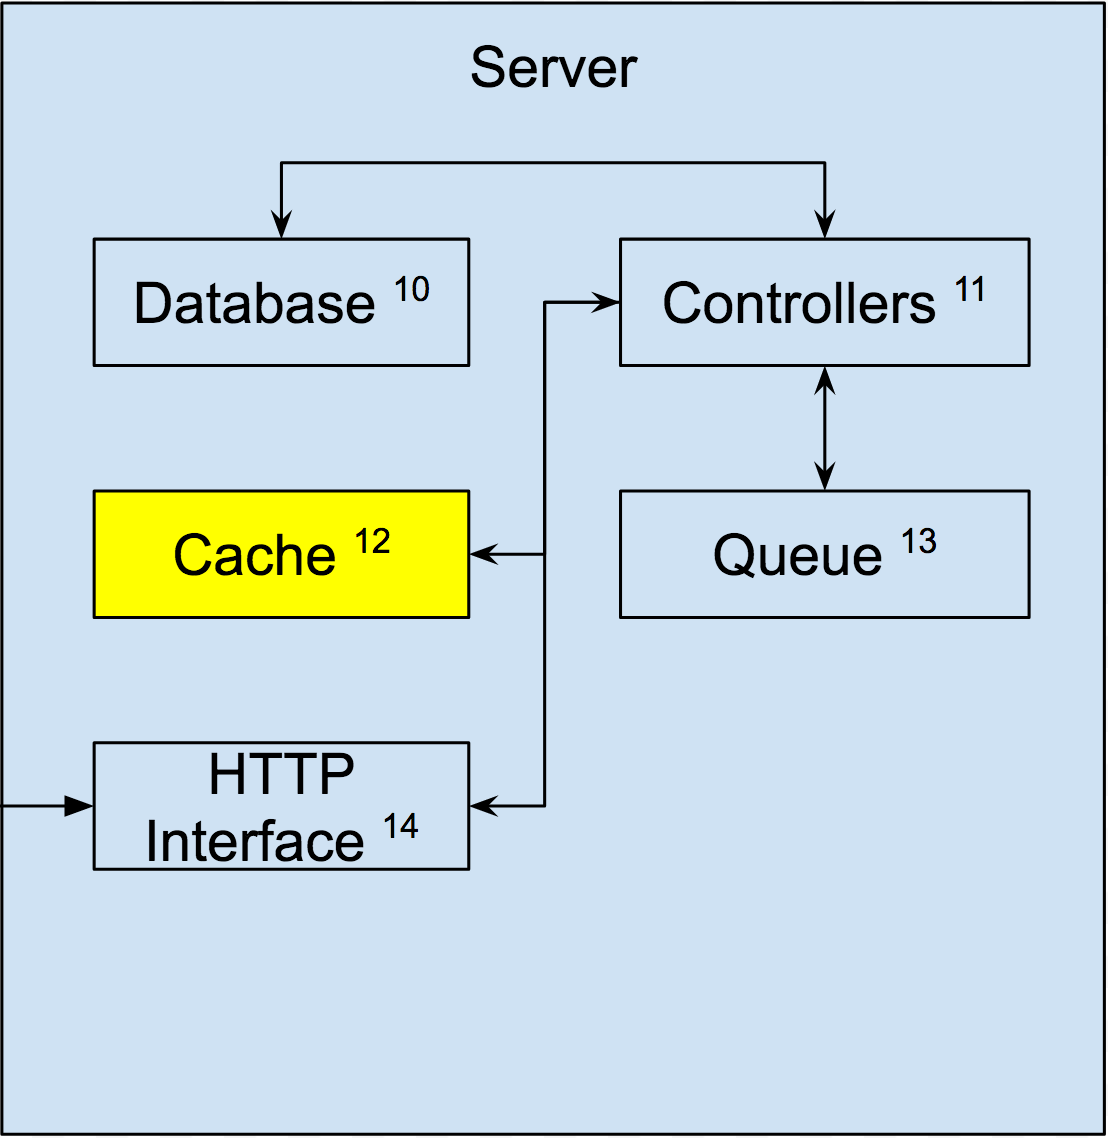
\includegraphics[width=0.60\textwidth]{images/server/server_cache.png}
 	\caption{Cache subsystem}
\end{figure}

\subsubsection{Assumptions}
N/A

\subsubsection{Responsibilities}
To save previous results

\subsubsection{Subsystem Interfaces}
\begin {table}[H]
\caption {Cache interfaces} 
\begin{center}
    \begin{tabular}{ | p{1cm} | p{6cm} | p{6cm} | p{6cm} |}
    \hline
    ID & Description & Inputs & Outputs \\ \hline
    \#01 & Make request & \pbox{3cm}{Retrieve song info} & \pbox{3cm}{Store song info in cache}  \\ \hline
    \end{tabular}
\end{center}
\end{table}

\newpage
